% REMEMBER TO SET LANGUAGE!
\documentclass[a4paper,10pt,english]{article}
\usepackage[utf8]{inputenc}
\usepackage{cite}
\usepackage{braket}
\usepackage{enumitem}
\usepackage{upgreek}
\usepackage{multicol}
\usepackage{mhchem}

% Standard stuff
\usepackage{amsmath,amsthm, amssymb,graphicx,varioref,verbatim,amsfonts,geometry,esint,url,color}
% colors in text
\usepackage[usenames,dvipsnames,svgnames,table]{xcolor}
% Hyper refs
\usepackage[colorlinks]{hyperref}
\usepackage{float}
\usepackage{wrapfig}
\usepackage{circuitikz}

\usepackage{tikz}
\usepackage[framemethod=tikz]{mdframed}
\usepackage{tikz-3dplot}
\usetikzlibrary{matrix,calc}

\usepackage{bm}

\usepackage[export]{adjustbox}

\usepackage{subfig}
\usepackage{algpseudocode}
\usepackage{algorithm}
\usepackage[makeroom]{cancel}

\usepackage{tcolorbox}
\tcbuselibrary{most}

%%%% PREVENT EXTRA WHITESPACE IN SECTION TITLES
\usepackage{sectsty}
\sectionfont{\raggedright}
%%%%

%%%%%FOR THE enumitem PACKAGE
\setlist[enumerate]{label*=\arabic*.}
%%%%%

%%%%EXAMPLE ENVIRONMENT

\newtcolorbox
[auto counter,number within=section]{pabox}[2][]{
%
enhanced,colback=black!5!white, colframe=black, fuzzy shadow={0mm}{-4pt}{-0.5pt}{0.4mm}{black!60!white},
title=Example 
\thetcbcounter
: #2,#1}

\newcommand{\example}[2]{
\begin{pabox}[label={myautocounter}]{#1}
#2
\end{pabox}
}
%%%%%%%%%%%%%%%%%%%%%%

%%%% BOX EQUATION ENVIRONMENT

\newenvironment{boxequation}{
\begin{tcolorbox}[ams equation, enhanced, colback=black!50!green!10!white, colframe=black, fuzzy shadow={0mm}{-4pt}{-0.5pt}{0.4mm}{black!60!white}]}
{\end{tcolorbox}}
%%%%%%%%%%%%%%%%%%%%%%%%%%%%%

%%%% BOX QUOTE ENVIRONMENT

\newenvironment{boxquote}{
\begin{tcolorbox}[enhanced, colback=black!50!green!10!white, colframe=black, fuzzy shadow={0mm}{-4pt}{-0.5pt}{0.4mm}{black!60!white}]
\begin{center}}
{\end{center}\end{tcolorbox}}

%%%%%%%%%%%%%%%%%%%%%%%%%%

% Document formatting
\setlength{\parindent}{0mm}
\setlength{\parskip}{1.5mm}


%Color scheme for listings
\usepackage{textcomp}
\definecolor{listinggray}{gray}{0.9}
\definecolor{lbcolor}{rgb}{0.9,0.9,0.9}

%Custom Math Operators
\DeclareMathOperator{\col}{col}
\newcommand{\colx}{\col x}

\DeclareMathOperator{\row}{row}
\newcommand{\rowx}{\row x}

\DeclareMathOperator{\nul}{nul}
\newcommand{\nulx}{\nul x}

\DeclareMathOperator{\rank}{rank}
\newcommand{\rankx}{\rank x}

\DeclareMathOperator{\Span}{span}
\newcommand{\Spanx}{\span x}

\DeclareMathOperator{\range}{range}
\newcommand{\rangex}{\range x}

\DeclareMathOperator{\dist}{dist}
\newcommand{\distx}{\dist x}

\DeclareMathOperator{\proj}{proj}
\newcommand{\projx}{\proj x}

\usepackage{listings}
\lstset{
	backgroundcolor=\color{lbcolor},
	tabsize=4,
	rulecolor=,
	language=python,
        basicstyle=\scriptsize,
        upquote=true,
        aboveskip={1.5\baselineskip},
        columns=fixed,
	numbers=left,
        showstringspaces=false,
        extendedchars=true,
        breaklines=true,
        prebreak = \raisebox{0ex}[0ex][0ex]{\ensuremath{\hookleftarrow}},
        frame=single,
        showtabs=false,
        showspaces=false,
        showstringspaces=false,
        identifierstyle=\ttfamily,
        keywordstyle=\color[rgb]{0,0,1},
        commentstyle=\color[rgb]{0.133,0.545,0.133},
        stringstyle=\color[rgb]{0.627,0.126,0.941}
        }
        
       
\newcounter{subproject}
\renewcommand{\thesubproject}{\alph{subproject}}
\newenvironment{subproj}{
\begin{description}
\item[\refstepcounter{subproject}(\thesubproject)]
}{\end{description}}


\definecolor{ubuntu_terminal_background}{RGB}{48,10,36}

\lstdefinestyle{DOS}
{
    backgroundcolor=\color{ubuntu_terminal_background},
    basicstyle=\scriptsize\color{white}\ttfamily
}

\lstnewenvironment{terminal}[1]
  {%
   \mdframed[backgroundcolor = ubuntu_terminal_background, innertopmargin = -0.4cm, innerbottommargin = -0.1cm, hidealllines = true, innerleftmargin = 0.2cm, innerrightmargin = 0.2cm]%
   \lstset{
     backgroundcolor=\color{ubuntu_terminal_background}, keywords={},
     basicstyle=\scriptsize\color{white}\ttfamily, frame = none, numbers=none
   }%
  }
  {\endmdframed}


%%%%%%%%%%%%%%  VECTORS TO BOLD
%\let\oldhat\hat
%\renewcommand{\vec}[1]{\mathbf{#1}}
%%%%%%%%%%%%%%  

%%%%%%%%%%%%%% UNIT VECTOR 
\newcommand{\uveci}{{\bm{\hat{\textnormal{\bfseries\i}}}}}
\newcommand{\uvecj}{{\bm{\hat{\textnormal{\bfseries\j}}}}}
\DeclareRobustCommand{\uvec}[1]{{%
  \ifcsname uvec#1\endcsname
     \csname uvec#1\endcsname
   \else
    \bm{\hat{\mathbf{#1}}}%
   \fi
}}
%%%%%%%%%%%%%
  
\usepackage{titlesec}

\titleformat{\chapter}[display]
  {\normalfont\bfseries\Large\raggedleft\color{black}}
  {\tikz[remember picture,overlay] \node[opacity=0.9,inner sep=0pt,anchor=north] at (current page.north){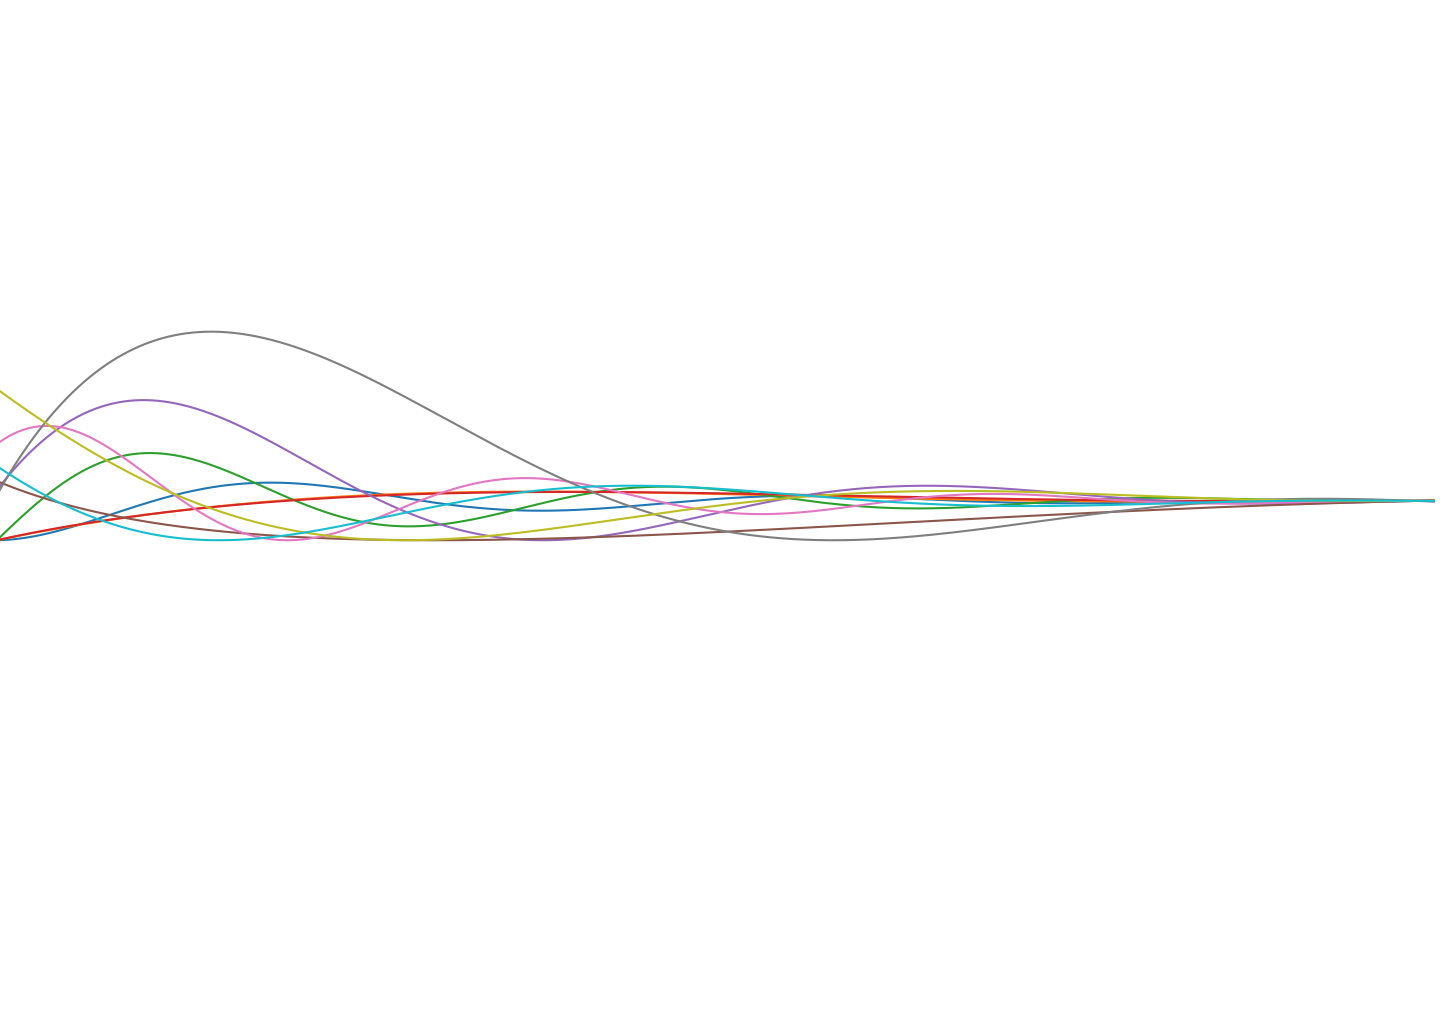
\includegraphics[width=\paperwidth,height=10cm]{header.png}};
    \MakeUppercase{\chaptertitlename}%
        \rlap{ \resizebox{!}{1.5cm}{\thechapter}}
  }
  {10pt}{\Huge}
\titlespacing*{\chapter}{0pt}{-30pt}{-5pt}

%Griffiths' style calligraphy font: use like $\scripty{r}$
\usepackage{calligra}
\DeclareMathAlphabet{\mathcalligra}{T1}{calligra}{m}{n}
\DeclareFontShape{T1}{calligra}{m}{n}{<->s*[2.2]callig15}{}
\newcommand{\scripty}[1]{\ensuremath{\mathcalligra{#1}}}

\begin{document}

\ctikzset{bipoles/length=.6cm}
\newcommand\esymbol[1]{\begin{circuitikz}
\draw (0,0) to [#1] (1,0); \end{circuitikz}}

\begin{titlepage}
	\centering
	{\scshape\LARGE \par}
	\vspace{1cm}
	{\huge\bfseries Obligatory Assignment 1 \par}
	\vspace{1.5cm}
	{\scshape\Large \par}
	\vspace{2cm}
	{\Large\itshape Gabriel Sigurd Cabrera\par}
	\vfill
	\textsc{stk-in}4300\vfill

% Bottom of the page
	{\large \today\par}
\end{titlepage}

\section*{Problem 2}

We are given the \textit{linearized} expression for the \textit{object function}:

\begin{equation}
\label{eq_0}
\mathbf{A} \equiv \sum_{i=1}^{N} g^\prime(\mathbf{w}_\text{old}^\textsc{t} \mathbf{x}_i)^2 \left( \frac{y_i - g(\mathbf{w}_\text{old}^\textsc{t} \mathbf{x}_i)}{g^\prime(\mathbf{w}_\text{old}^\textsc{t} \mathbf{x}_i)} + \mathbf{w}_\text{old}^\textsc{t} \mathbf{x}_i - \mathbf{w}^\textsc{t} \mathbf{x}_i \right)^2
\end{equation}

We are interested in minimizing $A$; to accomplish this, we must take the derivative of $A$ with respect to $\mathbf{w}$. We can then set this derivative to zero, and solve for $\mathbf{w}_\text{min}^\textsc{t}$.

To accomplish this, we must redefine (\ref{eq_0}) such that its \textit{summation notation} is replaced with a \textit{vector/matrix} expression; we begin by redefining some terms.  Let $p_i \equiv \frac{y_i - g(\mathbf{w}_\text{old}^\textsc{t} \mathbf{x}_i)}{g^\prime(\mathbf{w}_\text{old}^\textsc{t} \mathbf{x}_i)} + \mathbf{w}_\text{old}^\textsc{t} \mathbf{x}_i$, and let $q_i \equiv g^\prime(\mathbf{w}_\text{old}^\textsc{t} \mathbf{x}_i)^2$.  This gives us:

\begin{equation*}
= \sum_{i=1}^{N} q_i ( p_i - \mathbf{w}^\textsc{t} \mathbf{x}_i )^2 = (\mathbf{p} - \mathbf{w}^\textsc{t} \mathbf{x}^\textsc{t})^\textsc{t}\mathbf{q}(\mathbf{p} - \mathbf{w}^\textsc{t} \mathbf{x}^\textsc{t})
\end{equation*}

We then expand the above, giving us several easily-differentiable terms:

\begin{equation*}
= (\mathbf{p}^\textsc{t}\mathbf{q} - \mathbf{w} \mathbf{x} \mathbf{q})(\mathbf{p} - \mathbf{w}^\textsc{t} \mathbf{x}^\textsc{t}) = \mathbf{p}^\textsc{t}\mathbf{q}\mathbf{p} - \mathbf{w} \mathbf{x} \mathbf{q}\mathbf{p} - \mathbf{p}^\textsc{t}\mathbf{q}\mathbf{w}^\textsc{t} \mathbf{x}^\textsc{t} + \mathbf{w} \mathbf{x} \mathbf{q}\mathbf{w}^\textsc{t} \mathbf{x}^\textsc{t}
\end{equation*}

We can then differentiate the above with respect to $\mathbf{w}$:

\begin{equation*}
\frac{\partial \mathbf{A}}{\partial \mathbf{w}} =  -\mathbf{x} \mathbf{q}\mathbf{p} - \mathbf{p}^\textsc{t}\mathbf{q} \mathbf{x}^\textsc{t} + 2 \mathbf{x} \mathbf{q}\mathbf{w}^\textsc{t} \mathbf{x}^\textsc{t} = -2 \mathbf{x} \mathbf{q} \mathbf{p} + 2 \mathbf{x} \mathbf{q} \mathbf{w}^\textsc{t} \mathbf{x}^\textsc{t} 
\end{equation*}

\end{document}
